% !TEX program = XeLaTeX
% !TEX encoding = UTF-8
\documentclass[UTF8,nofonts]{ctexart}
\setCJKmainfont[BoldFont=FandolSong-Bold.otf,ItalicFont=FandolKai-Regular.otf]{FandolSong-Regular.otf}
\setCJKsansfont[BoldFont=FandolHei-Bold.otf]{FandolHei-Regular.otf}
\setCJKmonofont{FandolFang-Regular.otf}

\usepackage{url}
\usepackage{cancel}
\usepackage{xspace}
\usepackage{graphicx}
\usepackage{multicol}
\usepackage{multirow}
\usepackage{subfig}
\usepackage{amsmath}
\usepackage{amssymb}
%\usepackage[a4paper,width=180mm,top=18mm,bottom=22mm,includeheadfoot]{geometry}
\usepackage[a4paper,width=140mm,top=18mm,bottom=22mm,includeheadfoot]{geometry}
\usepackage{booktabs}
\usepackage{array}
\usepackage{verbatim}
\usepackage{caption}
%\usepackage{natbib}
\usepackage{booktabs}
\usepackage{float}
\usepackage{pdflscape}
\usepackage{mathtools}
\usepackage[usenames,dvipsnames]{xcolor}
\usepackage{afterpage}
\usepackage{pgf}
\usepackage{tikz}
\usepackage{dirtree}
\usepackage{amsfonts}
\usepackage{tkz-graph}
\newtheorem{definition}{定义}[section]
\newtheorem{theorem}{定理}[section]
\newtheorem{lemma}{Lemma}
\newtheorem{proof}{证明} [section]
\usepackage[toc,page,title,titletoc,header]{appendix}
\usepackage{marginnote}
\usepackage{tablefootnote}

\renewcommand\appendixname{附\ 录}
\renewcommand\appendixpagename{附\ 录}
\renewcommand\appendixtocname{附\ 录}

\usepackage{perpage} %the perpage package
\MakePerPage{footnote} %the perpage package command

\usetikzlibrary{shapes.geometric}%
\usepackage{color}
%\usepackage[pages=some,placement=top]{background}
\usepackage{eso-pic}

\title{\textbf{LOOPRING(路印)}\\\textbf{去中心化代币交易撮合协议}\\1.22版}
\author{
    daniel@loopring.org\\
    alex@loopring.org\\
    jay@loopring.org  \\
    \\
  \textit{Loopring Project Ltd}\\
%  \textit{https://loopring.org}\\
  \textit{foundation@loopring.org}\\
}

\makeatletter
\def\CTEX@section@format{\Large\bfseries}
\makeatother

\makeatletter
\newenvironment{tablehere}
  {\def\@captype{table}}
  {}

\newenvironment{figurehere}
  {\def\@captype{figure}}
  {}
\makeatother

%\newcommand\BackgroundPic{%
%\put(0,0){%
%\parbox[b][\paperheight]{\paperwidth}{%
%\vfill
%\centering
%
\includegraphics[width=\paperwidth,height=\paperheight,%
%%keepaspectratio]{images/background.jpg}%
%]{images/background.jpg}%
%\vfill
%}}}

\begin{document}
%\AddToShipoutPicture{\BackgroundPic}
\maketitle

本文仅供参考之用,不构成在任何司法管辖区出售证券或招揽购买证券的要约。 

\begin{abstract}
本文描述了一个开放的,支持类ERC20和智能合约的代币间多边交易协议。通过该协议,可以建立去中心化且无需资产托管的交易所应用。我们将该协议定位为下一代数字资产交易所的开放标准之一和架构基石。传统交易所可以通过拥抱该协议改进目前交易所的撮合方式,降低用户信任成本和自身运营风险;去中心化应用(dApp)也可以在智能合约中调用该协议提供的合约实现应用内的代币转换。

\end{abstract}

\newpage

\tableofcontents
\newpage

\section{背景\label{sec:background}}

区块链\cite{staff2016blockchains}\cite{swan2015blockchain}作为比特币\cite{nakamoto2008bitcoin}的底层技术,本质上是去中心化无信任环境中的存在性共识机制\cite{lamport1982byzantine}\cite{christidis2016blockchains}。存在性可应用于各种不同的数据,如股权,版权,使用权等。尽管联盟链和企业私有链中共识数据的类别正在变得越来越多样化,但这些数据的价值却有着明确的边界限制\ --- 只限于联盟成员间和企业内部。我们认为区块链的价值网络属性目前只有在公有链中才能得到更好的体现。根据coinmarketcap.com 的统计,截止本文成稿时间,区块链上代币总市值已经接近790亿美元,以太坊区块链\cite{wood2014ethereum}(ETH)上承载的代币市值也已超过170亿美元。

区块链对各行业都可能有着深远的影响,尤其是金融领域。我们相信基于区块链的新金融会有一个明显趋势,即资产代币化(Tokenization)\cite{liu2016medical}\cite{christidis2016blockchains}:一方面链下资产的使用权,所有权,分红权等相关权益通过抵押,会以代币(Token)\cite{swan2015blockchain}的形式发行到区块链上,另一方面区块链上资产也会进行跨链发行。资产代币化的目标之一就是低成本,全球化,全天候的高流动性。而流动性则主要通过交易所得以实现,因此一个更适合区块链上代币的交易标准对于区块链金融至关重要。

现阶段交易所都采用类似的模式:交易所要求用户将法币或者代币充值到交易所的银行账户或区块链地址中,然后交易所在自己的私有虚拟账户系统中为用户进行IOU记账。用户实际交易的是这些IOU。为了将IOU 兑换成法币或区块链代币,用户需要向交易所提出提现申请,提现成功后,才算真正交易完成。在这个过程中,交易所替用户保管资产的能力是用户最大的风险;同时用户还需承担交易所运营者商业道德带来的其它风险,比如挪用资金造成资不抵债等。2014年2月当时世界最大的比特币交易所Mt.Gox的85 万个比特币被盗一空\cite{mcmillan2014inside},公司向日本东京地方法院申请破产保护。该公司的用户至今仍在等待其返还尚未被盗的少量比特币。随着调查的不断进行Mt.Gox 被曝出所谓的比特币被盗其实是监守自盗。85万个“被偷窃”的比特币中,实际上因外部盗窃失踪的仅为7000个。2016年8月最大的美元比特币交易平台香港的Bitfinex由于网站出现安全漏洞,导致用户持有的比特币被盗,被盗的比特币共119756枚,总价值约为6500万美元。随后该公司决定由所有用户共同分担损失以避免破产。这些发生过的事件一方面反映出区块链代币交易在各个国家监管政策的缺失,另一方面也证实了中心化交易所模式的固有风险。

本文描述的基于区块链的去中心化交易机制就是为了彻底解决上述问题。去中心化交易的核心优势之一是避免任何资产被托管,因此资产就不存在被盗的可能,这会极大降低用户对交易所的信任成本。这种交易机制的另一个优势是没有地缘和时间限制,以及极高的透明性和可追溯性。这些特点会促使交易整体具有更大的流动性和更小的价差。

\section{相关工作\label{sec:existingworks}}

开源社区已经有过一些基于区块链搭建去中心化交易所的尝试,如瑞波(Ripple)、比特股(BitShares)、Openledger等。

Ripple \cite{schwartz2014ripple} 是一个去中心化的银行系统间清算协议,是为了解决银行间清算的高费用和高延迟问题而设计,具有快速、方便、超低费用的优点。Ripple提出了一项Interledger \cite{thomas2015protocol} 协议(ILP)实现跨账本的资产交易。ILP 本身并不是一个账本,相反,它提供了一个顶层加密托管系统,在称之为“连接者”的中介机构的帮助下,可以让资金在各账本之间进行流动。Ripple交易依赖于网关间信任的建立,而网关提供代币发行功能。

比特股(BitShares) \cite{schuhbitshares}\cite{schuh2015bitshares}  是一个区块链开发平台,任何个人和机构都可以在此平台上自由地进行转账、借贷、发行资产等,也可以基于这个平台快速搭建出去中心化的金融服务平台等。BitShares内置的去中心化交易所(DEX),让数字资产的交易撮合和交割完全发生在链上,并通过内置智能合约锚定其他资产,如法币、比特币、黄金、白银等。可惜BitShares项目由于开发者自身的问题,已经慢慢被边缘化。

Openledger\cite{openledger}是一个新型去中心化交易平台。它允许用户将比特币兑换成法币锚定的SmartCoins,SmartCoins可以直接通过paypal、瑞波网关兑换成现金。需要注意的是,Openledger在很大程度上依赖于BitShares 2.0平台以及Graphene Toolkit。因此,Openledger平台的性能取决于Graphene Toolkit的性能和BitShares 2.0平台的性能。

比特币的闪电网络\cite{poon2015bitcoin}和以太坊上的雷霆网络\cite{raidennetwork}是两个去中心化的系统。它们的卓越之处在于,无需信任对方以及第三方即可实现实时的、海量的交易网络。闪电网络和雷霆网络提供了一个可扩展的微支付通道网络。交易双方若在区块链上预先设有支付通道,就可以多次、高频、双向地通过轧差方式实现瞬间确认的微支付;双方若无直接的点对点支付通道,只要找到网络中一条连通双方的、由多个支付通道构成的支付路径即可。闪电网络和雷霆网络的突出贡献是将链上交易放到链外,只把最后一笔清算交易提交到区块链上,从而变相为区块链扩容。

Bancor\cite{bancor}协议引入了一种基于数学模型的方案去试图解决经济学中的“双重需求巧合”问题。其理念和预测市场中的Logarithmic Market Scoring Rules(LSMR)\cite{hanson2012logarithmic}类似。Bancor协议基于以区块链为基础的智能合约和储备代币,允许任何人通过这个协议创建代币,新的代币以预先设置的比率来持有一种或几种其它代币作为自己的储备金。这些储备代币可以是法币、数字化资产或其它加密代币。通过使用这些储备金,不论有没有交易,新创建的代币都可以获得价格,并随时可以兑换回其对应的储备代币。

0x \cite{warren20170x} 是一个可以在以太坊区块链上进行 ERC20\cite{ERC20} 代币对等交易的开放式协议。该协议旨在成为通用开放标准,作为可与其他协议组合的基本模块,用以驱动越来越复杂的区块链应用程序。由于它使用的是以太坊的智能合约系统,因此可以作为各种 dApps 的共享基础架构。而从长远来看,开放式技术标准相比封闭模式具有更大的优势,随着每个月有更多的资产在区块链上被代币化,也有更多的 dApps 需要使用这些不同的代币,开放式标准也因此变得更加重要。此外,由 dApps 耦合到其底层协议所导致的智能合约冗余也是未来区块链协议开发的主要障碍,因此在标准化之余,我们还需要一个合适的解耦方式。0x 协议试图将信息交换功能从应用层拉到协议层,推动dApps之间的互操作性。然而,0x协议的局限包括:taker必须在线匹配订单,这导致撮合实时性差,难以优化成交价格;0x协议采用的是简单的OTC 方式,无法法实现复杂订单的撮合;不同交易所之间没有明确的竞争激励机制;也没有考虑了矿工的利益。

上述努力由于种种限制,到目前为止依然没有能够撼动中心化交易所的地位。我们主要受到支付通道和0x 协议的启发,提出一种更可行的链上交易撮合标准。


\section{协议设计\label{sec:protocol}}

\begin{center}
\begin{figurehere}
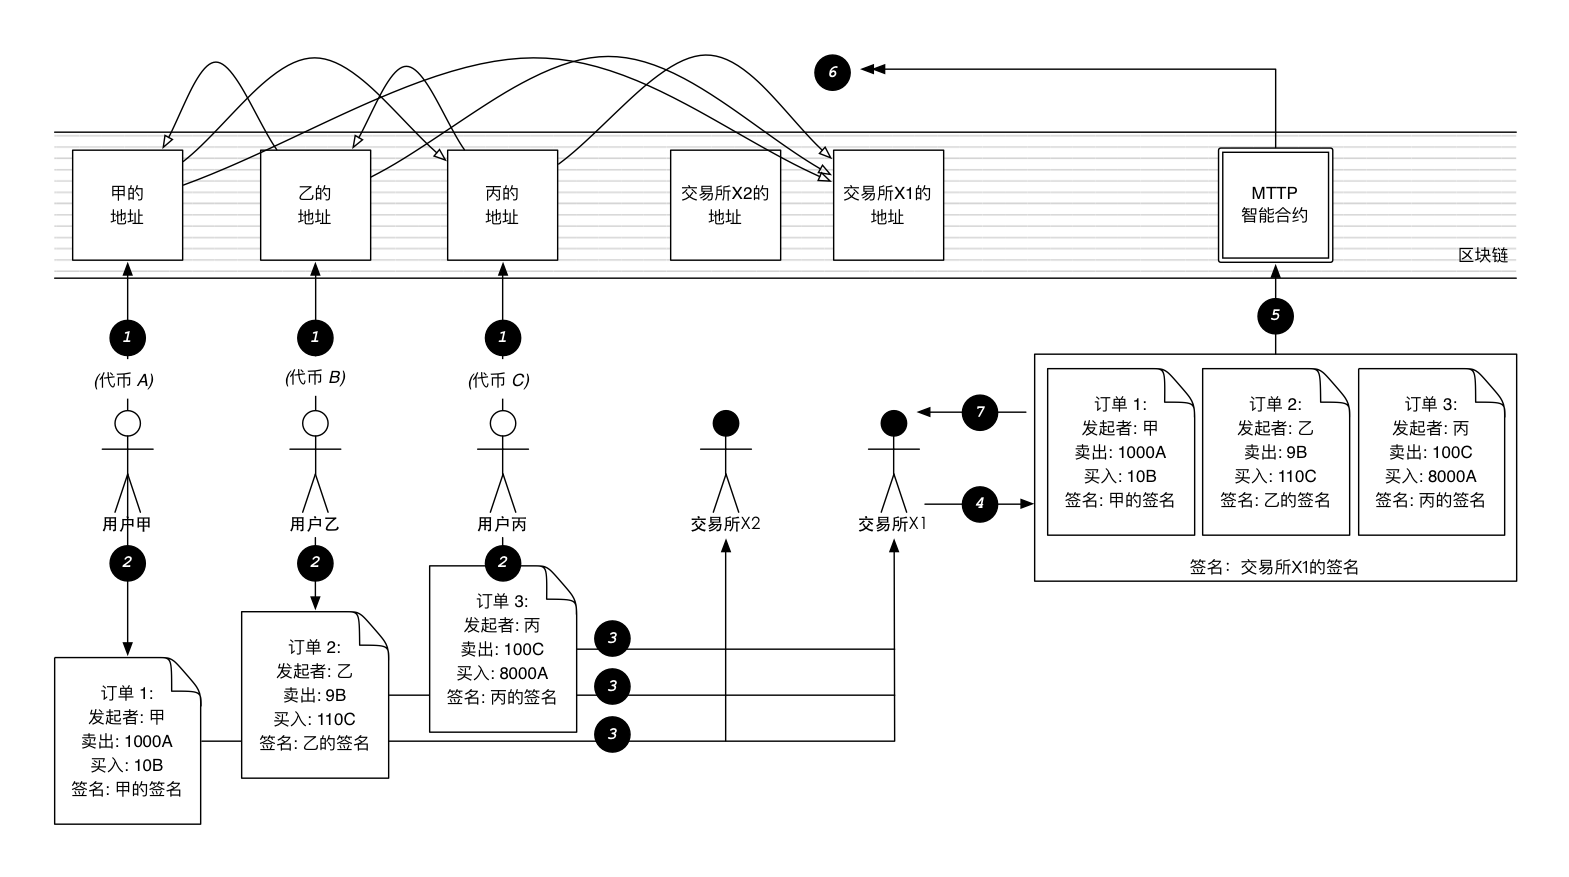
\includegraphics[height=8cm]{images/zh_protocol.png}
\caption{Loopring协议:图中示例一个三边交易的撮合}
\label{fig:Loopringprotocol}
\end{figurehere}
\end{center}

我们用上图中的三边交易,简要讲解下采用Loopring协议的撮合交易过程。该过程如下:

\begin{enumerate}
  \item 用户甲、乙、丙分别对Loopring撮合智能合约(Loopring Matching Contract)授权,授权后该合约可对用户指定代币账号做不超过一定额度的转出操作\footnote{通过ERC20机制实现。}。在上面实例中,合约可最多从用户甲的账号转出1000个$A$代币,从用户乙账户转出9个$B$代币,从用户丙账户转出100 个$C$代币;
  \item 用户甲、乙、丙分别生成自己的订单,并用私钥对其进行数字签名。订单不再区分买单和卖单,所有订单都被视为\texttt{交换单}\ --- 甲的订单声明:甲愿意卖出不多于1000个$A$代币,买到尽可能多但不少于10个$B$代币;如果是部分成交,那么$A$到$B$的\texttt{兑换率}不得低于1000/10 = 100.0(卖出代币数量除以买入代币数量)。订单中还可以包含其它参数,我们在章节\ref{sec:dataformat}中会对订单参数进行说明;
  \item 甲、乙、丙分别将自己的订单通过适当的方式发送到一个或多个交易所;
  \item 交易所收到上述三个订单,将它们分别放到三个对应的订单表(orderbook)中,并实时通过区块链数据更新计算每个订单的状态,同时不断努力寻找能够撮合的一组订单\ --- 我们后续称之为\texttt{交易环路}或者\texttt{撮合环路}。一旦确定三个订单的当前状态可以撮合成功,且收益满足预期,即决定实施这个撮合;
  \item 交易所对撮合交易签名后发送到Loopring撮合智能合约地址;
  \item 撮合智能合约验证四方签名,之后验证三个订单(的最新状态)是否可以真正成交。若无法成交,合约终止(交易所依然要消耗一定的油费);否则智能合约分别计算出甲、乙、丙三方各自需要支出的金额,以及交易所该收取的费用,并且实时将甲、乙、丙账号中的资产进行互转,并完成对交易所的费用支付 --- 如下图所示。在交易过程中,撮合智能合约还会调用Loopring注册智能合约(Loopring Registration Contract)来计算交易所应该给予该笔交易的费用折扣;在交易完成前,还会调用Loopring统计智能合约(Loopring Stats Contract)对交易所以及代币相关的统计数据做更新。

\begin{center}
\begin{figurehere}
\includegraphics[height=5cm]{images/zh-Loopring-example.png}
\caption{Loopring协议:交易环路结算}
\label{fig:Loopringprotocol}
\end{figurehere}
\end{center}
  
  \item 交易所监听新的区块和链下新的交易数据,并根据这些数据更新订单表,然后不断进行新的撮合。
\end{enumerate}





接下来我们介绍可以撮合成交的交易环路相关的概念,包括\texttt{交易链},交易链的可归约性,成交价,成交量,和交易所收益模型。

\subsection{符号定义}

在正式介绍协议之前,我们要介绍一些符号的定义。
\[
\begin{split}
&C_{i}\text{ :}\text{编号为$i$的代币币种。}\\
&O_{i\rightarrow j}\text{:}\text{一个卖出代币为$C_{i}$,买入代币为$C_{j}$的订单。}\\
&s_{i\rightarrow j}\text{:}\text{表示上述订单的当前卖出代币$C_{i}$的数量。}\\
&b_{i\rightarrow j}\text{:}\text{表示上述订单的当前买入代币$C_{j}$的数量。}\\
&r_{i\rightarrow j}\text{:}\text{为订单$O_{i\rightarrow j}$的兑换率,即$s_{i\rightarrow j} / b_{i\rightarrow j}$。}
\end{split}
\]


为了特指订单的原始状态,我们为符号加上水平线,代表其在原始订单中的值,比如$\overline{s}_{i\rightarrow j}$和$\overline{b}_{i\rightarrow j}$分别代表原始订单中的卖出和买入代币数量。

\subsection{订单兑换率恒定\label{sec:consistrate}}

除非订单完全成交,即$s_{i\rightarrow j} = 0$,否则Loopring协议保证订单状态更新后:
$s_{i\rightarrow j} / b_{i\rightarrow j}$ $=$ $\overline{s}_{i\rightarrow j} / \overline{b}_{i\rightarrow j}$,即订单中隐含的兑换率不会因为部分成交而变化,亦即$r_{i\rightarrow j} = \overline{r}_{i\rightarrow j}$。

在实际实施中,兑换率恒定是通过先计算部分成交后卖出代币的剩余量,再使用原始订单中隐含的兑换率来计算买入代币数量得以保证的。

\subsection{可规约性\label{sec:reducability}}


考虑两个订单$O_{i\rightarrow j}$和$O_{j\rightarrow k}$,我们可以通过中间代币$C_j$的连接,将其规约一个卖出代币为$Ci$,买入代币为$C_k$的订单。我们用$O_{i\rightarrow j\rightarrow k}$来表示这样一个订单,它和订单$O_{i\rightarrow k}$在撮合的各种属性上是等价的,且:

\begin{equation}
s_{i\rightarrow j\rightarrow k}=min(b_{i\rightarrow j},s_{j\rightarrow k}) \cdot r_{i\rightarrow j}
\end{equation}

\begin{equation}
b_{i\rightarrow j\rightarrow k}=min(b_{i\rightarrow j},s_{j\rightarrow k}) / r_{j\rightarrow k}
\end{equation}

\begin{equation}
r_{i\rightarrow j\rightarrow k}= r_{i\rightarrow j}\cdot r_{j\rightarrow k}
\end{equation}


在这里我们顺便引入\texttt{订单链}这个概念。一个订单链是两个或者两个以上订单,除了最后一个订单,每个订单的买入代币类型恰巧是后一个订单的卖出代币类型,但最后一个订单的买入代币类型不同于第一个订单的卖出代币类型(否则就成了一个环路)。我们可以将上述规约计算用于一个订单链。通过规约,一个包含$n-1$个订单($n$个不同的代币),即长度为$n-1$的订单链可被视为一个单一订单$O_{0\rightarrow ...\rightarrow n}$,且有:

\[ s_{0\rightarrow ...\rightarrow n} =
  \begin{cases}
    s_{0\rightarrow 1}      & \quad \text{如 } n \text{ = 1}\\
    min(b_{0\rightarrow ...\rightarrow n-1},s_{n-1\rightarrow n}) \cdot r_{0\rightarrow ...\rightarrow n-1}  & \quad \text{如} n \text{ $>$ 1}\\
  \end{cases}
\]

\[ b_{0\rightarrow ...\rightarrow n} =
  \begin{cases}
    b_{0\rightarrow 1}      & \quad \text{如 } n \text{ = 1}\\
    min(b_{0\rightarrow ...\rightarrow n-1},s_{n-1\rightarrow n}) / r_{n-1\rightarrow n}  & \quad \text{如} n \text{ $>$ 1}\\
  \end{cases}
\]


\[ r_{0\rightarrow ...\rightarrow n} = \prod_{i=0}^{n-1}{r_{i\rightarrow i+1}}
\]


订单链的可规约性可以帮助我们在分析订单路径时简化模型,在后文的讨论中,我们将符号$O_{i \rightarrow j}$的含义扩展到即包含简单的卖出代币为$C_i$,买入代币为$C_j$的单一订单,也包含可规约成这样一个类型订单的订单链,如果为了强调是个订单链,我们会用$O_{i \rightarrow ...\rightarrow j}$或$O_{i \rightarrow \rightarrow j}$表示。

\subsection{环路撮合}

传统撮合系统是在两个币种间,即一个交易对的买卖两个方向间完成撮合;而Loopring 协议将撮合的概念扩展到多币种,通过\texttt{交易环路}来完成多个币种之间交易的撮合。下面介绍一下交易环路的概念。

\begin{definition}[交易环路]
如果有$n$个币种$C_{0}$、$C_{1}$、$\cdots$、$C_{n-1}$,和$n$个订单:$O_{0\rightarrow 1}$, $\cdots$, $O_{i\rightarrow i\oplus 1}$, $\cdots$, $O_{n-1 \rightarrow 0}$,其中,$i\oplus 1 \equiv i+1 \mod n$。
那么这些订单可以组成跨n个币种的交易环路:

$O_{0\rightarrow 1} \rightarrow \cdots \rightarrow O_{i\rightarrow i\oplus 1} \rightarrow \cdots \rightarrow O_{n-1\rightarrow 0}$ ,其中$n$为环路的长度。
\end{definition}

当这些订单的价格\textbf{满足一定条件时},我们可以对整个交易环路进行撮合,这种交易环路称为\textbf{可交易环路}。下面我们对交易环路中的成交价格和成交量进行讨论。


\subsubsection{成交条件和价格\label{sec:matchprice}}

我们由一个长度为3的交易环路为例,介绍环路可成交的条件。假定环路中的三个币种为$C_{0}$、$C_{1}$ 和$C_{2}$,三笔订单分别为:$O_{0\rightarrow 1}$、$O_{1 \rightarrow 2}$和$O_{2 \rightarrow 0}$。很容易证明,如果$r_{0 \rightarrow 1} \cdot r_{1 \rightarrow 2}\cdot r_{2 \rightarrow 0} = 1$时,三个订单都可以用其自身的兑换率成交。当$r_{0 \rightarrow 1} \cdot r_{1 \rightarrow 2}\cdot r_{2 \rightarrow 0} > 1$时,三个订单都可以用比自身兑换率更低的兑换率成交。我们称第一种情况为\texttt{原价撮合},称第二种情况为\texttt{折价撮合}。

Loopring协议要求交易环路的折价平均分享给环路中的每个订单。假设每笔订单兑换率折价比例为$\gamma$,那么最终完成撮合时,三笔订单的成交价分别为:$r_{0\rightarrow 1} \cdot (1-\gamma)$,$r_{1\rightarrow 2} \cdot (1-\gamma)$,$r_{2 \rightarrow 0} \cdot (1-\gamma)$,并且满足:
\begin{equation}
r_{0\rightarrow 1} \cdot (1-\gamma)\cdot r_{1\rightarrow 2} \cdot (1-\gamma) \cdot r_{2 \rightarrow 0} \cdot (1-\gamma) = 1
\end{equation}

根据上式我们可以推导出:
\begin{equation*}
\gamma = 1- \frac{1}{\sqrt[3]{r_{0\rightarrow 1} \cdot r_{1\rightarrow 2} \cdot r_{2\rightarrow 0}}}\text{。}
\end{equation*}

在更一般的情形下,如果跨$n$个币种的环路中,\texttt{兑换率折扣}为:
\begin{equation*}
\gamma = 1- \frac{1}{\sqrt[n]{\prod_{i=0}^{n-1} r^i}} \text{,其中} r^i \text{表示第}i\text{个订单的兑换率。}
\end{equation*}

显然,只有在兑换率折扣$\gamma \ge 0$时,交易环路才可以真正成交;且第$i$ 个订单$O^i$的实际兑换率$\hat{r^i} = r^i \cdot (1-\gamma)$,且有$\hat{r^i}\le r^i$。

%在章节\ref{sec:fee}中,我们还会详细介绍交易所通过Loopring代币抵押的原因和细节,最终的结果是每个交易都被迫给自己的撮合的实际兑换率打个折扣,即\texttt{交易所折扣}。假交易所$X$的交易所折扣为$\mu$,那么由该交易所撮合是,最后的实际成交兑换率为:$\hat{r^i} = r^i \cdot (1-\gamma) \cdot (1-\mu)$


\subsubsection{成交量\label{sec:matchquantity}}

当一个交易环路撮合完成后,至少有一个订单是被完全成交的。这点很容易得到证明:我们可以先假设该结论不成立,即全部订单都没有完全成交。由于章节\ref{sec:consistrate}中要求兑换率在订单新状态(尾单)中保持不变,意味着撮合后新的环路依然满足成交条件。这就意味着之前的撮合是没有进行完的。因此可以断言:一次完整的撮合应该会将至少一个订单完全吃掉。我们称这个(些)被完全吃掉的订单为交易环路的\texttt{最小订单}。

找到任何一个最小订单,既可循环计算环路中所有订单的成交量。假设第$i$个订单是最小订单,那么每笔订单的卖出代币成交量$\hat{s}$和买入代币成交量$\hat{b}$可以以此如下计算得出:

\[
\begin{split}
&\hat{s}^{i}=\overline{s}_i\text{,} \hat{b}^{i}=\hat{s}^{i} / \hat{r}^i \text{,其中}\overline{s}_i\text{为订单的卖出代币余额;}\\
&\hat{s}^{i\oplus 1}=\hat{b}^i\text{,} \hat{b}^{i\oplus 1}=\hat{s}^{i\oplus 1} / \hat{r}^{i\oplus 1}\text{;}\\
&\hat{s}^{i\oplus 2}=\hat{b}^{i\oplus 2}\text{,} \hat{b}^{i\oplus 2}=\hat{s}^{i\oplus 2} / \hat{r}^{i\oplus 2}\text{;}\\
& ...
%\text{。}
\end{split}
\]

实际实施过程中,可以先假定第一个订单为最小订单,往后循环计算成交量,直到每个订单的成交量都不再变化为止。理论上最多循环两次即可计算出每单的实际成交量。

\subsubsection{撮合费用\label{sec:fee}}

交易所第一种收费形式是手续费。在订单中可以设置一个以Loopring的代币 $LRC$为单位的费用, $m^i$,代表完全成交情况下编号为$i$订单愿意支付给交易所的手续费总和。实际成交时候按订单卖出代币成交比例支付给交易所,即:

\begin{equation*}
f^i = b^i \cdot m^i  / \overline{b^i}
\end{equation*}


为了鼓励交易所为用户找到兑换率折价比例最大的成交环路,Loopring协议要求将兑换率折价带来的\texttt{成本节约}分润给交易所。对与一个订单$O^i$, 假设买入订单的成交额度为$b^i$($b^i \le \overline{b^i}$),我们定义成本节约为:

\begin{equation*}
\Delta^i = b^i \cdot r^i \cdot \gamma
\end{equation*}

Loopring协议允许每个订单设定一个成本节约分享\texttt{分润比例} $\theta^i$,并将交易环路上所有订单分润比例的最小值作为该环路的分润比例$\Theta$,那么订单$O^i$ 支付给交易所的费用为:


\begin{equation*}
f^i = \Delta^i \cdot \Theta = b^i \cdot r^i \cdot \gamma \cdot \Theta
\end{equation*}

因此交易所对于一个交易环路,通过成本节约分润获得的收入为:

\begin{equation*}
F = \sum^{n-1}_{i=0} b^i \cdot r^i \cdot \gamma \cdot \Theta
\end{equation*}

采用所有订单中最小的分润比例作为整个交易环路的分润比例,可以激励订单采用较大的分润比例。这样做会激励交易所对订单进行撮合,同时一旦订单成交,也不一定非要支付指定比例的分润。


为了鼓励Loopring 的代币$LRC$ 的使用,如果订单中没有指定代币费用$m^i$,或$m^i=0$,那么该笔订单的分润比例实际被认为是100\%,而不管订单中相应参数的值是多少。如果一个交易环路中的所有订单都没有设置代币费用,$\Theta=100\%$,环路中所有成本节约归交易所所有。


在下一章节,我们会引入一个激励交易所竞争的代币抵押机制,智能合约根据每个交易所代币抵押数量的排名,为每个交易所计算一个\texttt{费用强制折扣},$\lambda$,该折扣会进一步影响交易所的费用收取;同时,交易所也可以指定为某个交易环路做进一步的费用优惠折扣,$\eta$。因此,交易所对于一个交易环路的整体费用为:

\begin{equation*}
F =(1-\lambda)\cdot (1-\eta) \cdot  \sum^{n-1}_{i=0} (b^i \cdot r^i \cdot \gamma \cdot \Theta + b^i \cdot m^i  / \overline{b^i})
\end{equation*}


两种不同的费用模型能够满足不同订单的诉求:对于没有$LRC$ 代币的账户,可以设置合适的分润比例;对于有$LRC$ 代币的账户,可以选择支付较多的代币费用,并将分润比例设为一个较小值。交易所有可能对每笔订单的代币费用值有个最小额度限制,Loopring协议并不对此作出明确要求。交易所可以在自己网站上对相关标准做说明,并引导用户设定合适的订单参数值。

\subsubsection{交易所费用强制折扣}
Loopring 协议要求交易所给交易费强制打一个折扣,折扣大小决定于交易所抵押$LRC$ 代币数量的排名,排名越靠后,折扣越高。假定排名为$n$的折扣为:

$$\lambda_{n} = 0.05\cdot(\ln (n+e-1) - 1)\text{。}$$
具体返利比例如下表所示:


\begin{table}[hbt]
  \centering
\begin{tabular}{p{3.5cm}|p{3cm}} %设置了每一列的宽度,强制转换。
抵押排名$n$ & 费用强制折扣$\lambda$ \\ %用&来分隔单元格的内容 \\表示进入下一行
    \hline
1 & 0\%\\
\hline
2 & $1.57\%$\\
\hline
10 & $7.31\%$\\
\hline
20 & $10.39\%$\\
\hline
99 &$18.06\%$\\
\hline
100 &$18.11\%$\\
\hline
1000 &$29.55\%$\\
\hline
1001 &$30.00\%^*$\\
  \end{tabular}
\caption{抵押$LRC$排名与费用强制折扣} %显示表格的标题
\end{table}


对于排名1001及以后的交易所,或未进行抵押的交易所,统一实施30\%费用强制折扣。

如下图所示,费用强制折扣的下降并非线性的,如$\lambda_{2} - \lambda_{1} \gg \lambda_{100} - \lambda_{99}$。

\begin{center}
\begin{figurehere}
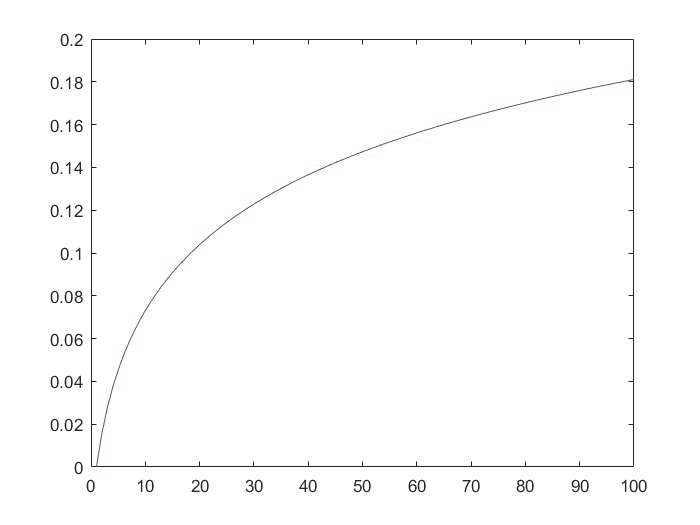
\includegraphics[height=8cm]{images/exchange-discount.png}

\caption{$LRC$代币抵押排名与费用强制折扣}
\label{fig:discount}

\end{figurehere}
\end{center}

在实际部署时,折扣函数中的参数需要根据市场行情不断调整,比如交易量和实时性。当市场交易量过于旺盛时,会导致过多交易无法及时确认,这时需要降低整体折扣率,尤其是原本折扣率高的那些交易所。当交易量低时,需降低折扣率,刺激交易的撮合。

\subsection{防作弊和防攻击}

\subsubsection{交易所无风险套利}
Loopring协议致力寻求在用户和交易所间利益的平衡点,打造公平健康的交易所生态。Loopring协议不反对交易所的套利行为,因为套利行为本质上也是在促成交易。但是我们禁止交易所利用自己在生态中角色的特殊性进行套利,具体来说,通过上传一种特殊的闭环无风险套取订单间的价差,本节我们将介绍如何防止交易所的这种行为。在介绍之前,我们首先来分析交易所如何做到无风险套利。

假设有两个订单$O_{a\rightarrow b}$,$O_{b\rightarrow a}$,形成一个交易环路,且$r_{a\rightarrow b} \cdot r_{b\rightarrow a} > 1$。交易所可以在这个环路上插入三个自己新生成的订单$O_{b\rightarrow c}$,$O_{c\rightarrow d}$,$O_{d\rightarrow b}$,生成一个长度为5
的新环路,并使$r_{a\rightarrow b}  \cdot r_{b\rightarrow c} \cdot r_{c\rightarrow d}\cdot r_{d\rightarrow b}\cdot r_{b\rightarrow a}  = 1$。通过这种方式,交易所可以做到将所有可能的成本节约变成0,一旦撮合被智能合约接受,即可实现无风险套利。

这种套利的交易环路有个显著的特征:它们包含子环路。在上个例子中,两个子环路分别是:$O_{a\rightarrow b}\rightarrow O_{b\rightarrow a}$和$O_{b\rightarrow c}\rightarrow O_{c\rightarrow d}\rightarrow O_{d\rightarrow b}$。为了杜绝交易所的这种无风险套利,Loopring协议要求:{\bfseries 合法的闭环必须保证其订单子集无法组成更小的可交易环路}。

\subsubsection{交易所拒绝服务}

Loopring协议允许交易所选择性地为特定订单做撮合。交易所有权对订单的代币类型,订单数量,费用等做筛选,也有权对这些筛选条件做更改,且有权公开或隐藏这些筛选条件。交易发起者与交易所之间是相互选择的关系,彼此没有任何义务。

\subsubsection{尘埃订单攻击}
普通用户可以通过广播大量的尘埃订单(即数量非常小的订单)试图对交易所做攻击,不过由于撮合尘埃订单获利很低,所以这些订单一定会被交易所抛弃,进而对交易所和区块链没有任何影响。

交易所也可能采用同样方式发起攻击,从而试图影响其它交易所对某些订单的撮合。不过这种努力也不会奏效,因为协议允许同一个订单在同一个块中参与到多个环路成交(这些环路可能是不同交易所提交到区块链上的),换句话说,订单并没有所谓的锁定状态。

\subsubsection{余额不足订单攻击}

交易发起者可能发起多笔订单,但订单卖出代币账户实际余额为零。这样的订单提交到交易所后,交易所很容易通过查询区块链地址的余额信息将该订单抛弃,不过这种攻击的确会浪费交易所的处理时间。好在交易所可以通过黑名单机制,迅速有效地将某些地址屏蔽掉,拒绝再为这些地址提供撮合服务。

\subsubsection{撮合窃取}

一个懒惰交易所可以监听网络上未被确认的撮合交易,解析交易环路并生成一个带有自己签名的新撮合(环路相同,只有受益地址和数字签名不同),通过提供更高的交易费来窃取其它交易所的撮合结果。特别当窃取者是矿工时,这种作弊行为是比较难以预防的。为防止撮合窃取,我们规定交易所上传订单环路的过程分为两步:
\begin{itemize}
    \item 交易所在区块链上发一笔交易,上传订单环路的存证,
    \item 存证信息被写入区块链后,交易所提交具体环路信息。
\end{itemize}
这个存证通过哈希来实现,哈希值的生成方法为
$$h = H(r, nonce)\text{,}$$
其中,$H()$为单向函数,$r$为订单环路信息。哈希函数的输入包含了一个随机数$nonce$,用于防止对哈希值进行暴力破解。在提交具体环路信息时,随机数$nonce$需要一并提交。

\subsection{市场深度\label{sec:marketdepth}}

交易所并不一定需要提供市场深度数据。在整个生态中,可能会有单独的组织和机构汇集全网的未成交订单或者交易的尾单信息,汇总成独立的市场深度数据。市场深度数据可以根据章节\ref{sec:reducability}中的订单的规约方法,计算出任何两个ERC20 代币之间的买单卖单数据。

\subsection{数据格式\label{sec:dataformat}}

由于采用OTC模型,所有订单可以用同一个数据结构表示。该结构包含订单本身的各种参数数据和发起者的数字签名。在签名前,先将订单参数数据连接成一个字节数组,通过Keccak SHA3方法对这个字节数组做散列计算得到订单的哈希,之后用账户私钥对这个哈希进行ECDSA签名。


\begin{verbatim}
message Order {
  address protocol;   // Loopring协议入口智能合约地址
  address owner;      // 该订单发起者地址
  address outToken;   // 卖出ERC20代币智能合约地址
  address inToken;    // 买入ERC20代币智能合约地址
  uint256 outAmount;  // 卖出ERC20代币数量上限
  uint256 inAmount;   // 买入ERC20代币数量下限
  unit256 expiration  // 过期时间
  unit256 fee;        // 交易总费用(LRC),部分成交的费用按该次
                      // 撮合实际卖出代币额与outAmount比例计算
  uint8 savingShare;  // fee不为0时支付给交易所的分润比例,否则视为100%
  unit8 v;
  bytes32 r;
  bytes32 s;
}
\end{verbatim}

订单中虽然没有明确指定价格,但我们可以通过计算$outAmount / inAmount$ 来得到一个订单兑换率$r$。该兑换率隐含地要求所有实际撮合成交的兑换率不得大于$r$。 一个好的交易所UI应该允许用户输入$outAmount$,$inAmount$,和传统意义的买入价或卖出价这三个数据的任意两个来计算缺失的$outAmount$或$outAmount$值。

订单实际上可以有两种不同的\texttt{完全成交}定义:一种定义是只有卖出代币达到了$outAmount$ 就算完全成交;另一种定义在之前的基础上允许买入代币累计金额达到$inAmount$也算完全成交。我们可以在订单中引入一个参数告诉交易所和撮合智能合约选择哪种完全成交定义。在第一版本的实现中,我们先支持第一种完全成交定义。


交易所可以通过下面的数据结构构建一个交易环路:
\begin{verbatim}
message MatchRing {
    Order[] orders;             // 该次匹配的所有订单
    address feeRecipient;       // 费用收取地址
    unit256 additionalDiscount; // 在费用基础上进行的再折扣价 - eta
    unit256 nonce;              // 一个随机数
    unit8 v;
    bytes32 r;
    bytes32 s;
}
\end{verbatim}

一个可交易环路上同一位置的订单只能有一个\ --- 理论上可以将这个限制去掉,不过这会让撮合智能合约更加复杂,我们可能在后续的版本中再给与支持。

\subsection{订单状态\label{sec:orderstate}}

订单发起者对订单签字广播后无法对该订单进行修改。撮合智能合约一旦对某个订单进行撮合,就需要在区块链上对订单的状态更新记录。对部分或者完全成交的订单,会计算更新$inAmount$和$outAmount$ 两个值,并且保障订单新状态价格和原始订单的价格一致。如果$inAmount$或$outAmount$为0,则表示该订单已经完全成交。如果用户取消订单,需要发起一个特殊的交易,将$inAmount$和$outAmount$更改为0即可。过期的订单不会触发区块链上的数据更新\ --- 可以根据最后一个块的时间戳来判断任何一个订单是否过期\ --- 因此我们期待多数的订单会因为过期或者完全成交而变成失效。

交易所需要采用同样的甚至是更复杂的逻辑在区块链外追踪订单状态,尤其是当一家交易监听到到竞争对手在对同一个订单做不同的撮合的时候。


一个可交易的订单还需要其账户中有足够多的卖出代币余额$balance$,虽然 $balance$ 不要求达到订单中$outAmount$的数量。实际上交易所在对订单状态计算的时候,会取$max(balance, outAmount)$ 作为实际的可成交金额。这里可以看出,订单的卖出代币并不需要锁定的过程。用户提交订单后依然可以任意支配卖出代币作为他用。交易所不仅仅要监听订单被(其它交易所)撮合的结果,还需要监听订单账户的余额变动情况。看起来这种对区块链数据的监听和对订单状态的更新有些复杂,但这些反而极大简化区块链上合约的逻辑,这种思路和比特币闪电网络,以太坊的雷霆网络的思路是一致的。

\subsection{智能合约\label{sec:contracts}}

Loopring协议协议可能包含多个智能合约,包括但不限于:

\begin{itemize}
  \item  \textbf{撮合合约} 负责计算并确认交易环路中每个订单的状态,计算成交金额和成交量,对交易进行清算转账。该合约还会与其它合约交互,是Loopring协议的入口合约;
  \item   \textbf{订单合约} 负责更新订单状态以及对取消订单提供支持;
  \item  \textbf{交易所注册合约}  负责维护和更新一系列支持Loopring协议的交易所,为交易所代币抵押和预设参数默认值提供支持;
  \item \textbf{统计合约}  计算任何两个币种之间的成交量,成交价,以及不同交易所的贡献度等指标,以及这些指标的某些滑动平均值。这些指标是订单发起者授权撮合的重要参考依据,同时也可以作为某些预测市场的输入,并且为以后可能的协议拓展(比如对条件单的支持)提供输入(Oracle)。

\end{itemize}

这里,不排除将上述合约进一步拆解或合并的可能。同时值得指出:Loopring协议中的智能合约是完全开放的,这意味着它们可以被任何的dApp 直接或者间接调用。因此整个协议即使一个完善的整体,又是个开放的,单独可用的组件的集合。

\begin{comment}
\subsection{支持ENS\label{sec:registration}}

以太坊提供通过名字解析地址的以太坊名字服务(Ethereum Name Service, ENS)\cite{hirai2016formal}。我们可以通过使用ENS,将Loopring协议中所有的智能合约,ERC20 代币发行地址,交易所收益地址等地址信息映射到相应的名字,一方面可以降低订单信息出错的可能性,另一方面也会减小订单和撮合交易的字节数。
\end{comment}

\section{Loopring协议代币$LRC$\label{sec:protocoltoken}}


我们将为Loopring协议发行符合ERC20规范的原生代币,其符号为$LRC$(在本文中用斜体字母表示)。


\subsection{代币的应用}

$LRC$在生态中发挥下列作用:

\begin{itemize}
  \item \textbf{作为撮合费用} --- 订单中可以指定用$LRC$可作为支付给交易所的撮合费用。虽然协议支持通过卖出代币成本节约的分润作为支付手段,但对于交易所来说,将来需要支持的ERC20代币类型可能越来越多,如果每笔撮合交易都通过各订单中的卖出代币为单位支付手续费,那么对于一次撮合的收益计算将变得复杂;相反,如果通过$LRC$来衡量收益(或者用来计算成本),会简单得多。同样,对于订单发起者,可以通过公开信息获取某笔订单需要支付大约多少费用,如果用每个订单的卖出代币计算,那么下单过程中的费用计算也会比较分散。我们在之前章节\ref{sec:fee}对费用模型做了详细的说明。
  \item \textbf{作为交易所注册抵押} ---订单发起者希望自己的订单得到最好的撮合,这要求交易所在各个方面都做到专业,特别是对全部订单的汇聚情况。由于去中心化交易没有地域限制,一个好的交易所应该能比一个相对差的交易所看到更多的订单,也应能在最短时间内找到最好的交易环路。为了鼓励实力强的交易所,淘汰实力差的交易所,我们提供一种交易所注册抵押机制:交易所可以将一定数量的$LRC$代币抵押给智能合约。交易所可以随时申请抵押代币的解冻,但申请提出后,一年后才锁定的代币才可以转账出去。并不是所有交易所都必须进行注册抵押。交易所代币抵押的另一个作用是防止交易所为了抛弃不利的历史统计数据而频繁变动身份。
\end{itemize}

\subsection{去中心化自治}
随着交易所的不断升级,交易所中的规则需要不断升级升级,为此我们引入去中心化自治机制。任何持有$LRC$者都可以将代币抵押并获得自治系统的投票权益,投票权益S是一个关于抵押数量N和抵押时间CoinAge 的函数,
$$S = f(N, CoinAge)\text{,}$$
其中 $CoinAge = H_{c}-H_{s}$,这里的CoinAge是当前区块高度$H_{c}$减去开始抵押区块高度$H_{s}$。加入CoinAge参数是为了防止有攻击者短时间内租借到大量代币并获得很高的权益,迫使某项并不为他人接受的提议得以通过。

在去中心化自治系统中,任何决定都要在一个固定时间内完成投票,这个时间根据提议内容不同而发生改变。当且仅当收集到足够高权益的投票,提议才会执行,否则提议将会关闭。在去中心化自治系统中,并不是权益高者的一言堂,权益低者可以联合在一起制衡权益高者。

去中心化自治内容包括但不限于交易所注册、币种注册、统计函数、抵押代币范围等,这些升级可以通过自治系统参与者共同投票参与决定。
  \begin{itemize}
    \item \textbf{币种注册} Loopring协议会阶段性的调整支持的币种,有些数字货币会因为交易量过低而退出交易所,而另外会有一些新的数字货币诞生而加入交易所。这些币种需要记录在智能合约中,包括币种名称、代号及对应智能合约地址等信息。
    \item \textbf{交易所注册} 交易所需要注册完成才能通过协议进行交易,当交易所达到一定数量后,新注册交易所需要经过自治系统投票才能通过。
    \item \textbf{统计函数} 随着交易所上线运行时间越长,数据量得到一定积累,用于统计的指标和函数也会逐渐成熟。自治系统参与者可以决定新增或淘汰统计函数。
    \item \textbf{抵押代币范围} 交易所可以抵押的代币数量需要限制在一定范围内。如果抵押数量太多,会导致代币流动性变差;如果抵押过少,则无法体现交易所间的差异性。
    \item \textbf{环路最大长度} 理论上说,环路越长越有可能发现利差大的环路,然而过长的环路会降低环路撮合的成功率,并且在过长的环路会带来过高的计算成本。
    \item \textbf{强制折扣函数} 强制折扣函数需要根据市场行情不断调整,比如交易量和实时性。当市场交易量过于旺盛时,会导致交易过多而无法及时确认,这时需要降低整体折扣率,尤其是原本折扣率高的那些交易所。当交易量低时,需降低折扣率,刺激交易的撮合。如下图所示,其中蓝色为交易量正常时的折扣率,黄色为市场交易量过高时的折扣率,红色为交易量过低时的折扣率。
\begin{center}
\begin{figurehere}
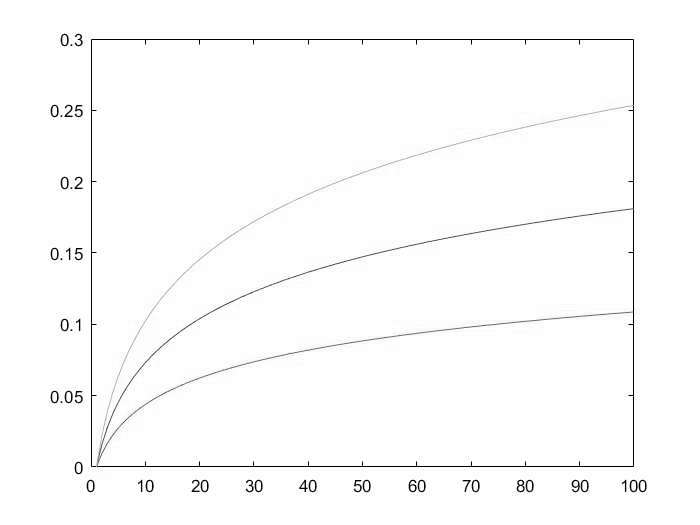
\includegraphics[height=10cm]{images/rate_adjust.jpg}
\caption{调整后的强制折扣率}
\label{fig:dischargeRateAdjust}
\end{figurehere}
\end{center}

    \item \textbf{子合约地址} 如果基于公有链搭建Loopring交易所,智能合约本身是无法改动的。在这种情况下,如果升级Loopring协议的子合约,则需要重新部署智能合约,并修改子合约的地址。
  \end{itemize}

%\footnotemark

\subsection{代币的原生流动性}

Loopring协议代币本身遵循ERC20标准,并且在Loopring智能合约的基础上带有原生的流动性\ --- 这意味着你不必去传统的交易所购买和出售$LRC$,而是可以通过本文论述的方式,利用Loopring协议本身的去中心化撮合机制,使用任何ERC20代币购得$LRC$(订单中的买入代币设定为$LRC$,并将$fee$设为0)。这得益于协议灵活的收费模式。


\section{交易所\label{sec:exchange}}

采用Loopring开放协议后,交易所并不能保证每一个撮合都是盈利的。一方面可能是成本过高,因为交易所为了激励矿工优先打包自己的撮合交易到区块链,可能根据预期的收益调高手续费,而手续费代币和撮合中代币的相对价格有可能有超出预期的浮动,从而造成手续费实际成本更高。另一方面可能是因为收入没有达到预期,比如交易所把撮合广播到区块链后,该撮合的某个订单的卖出代币被部分或者全部转移到另一个地址,从而造成整个撮合交易未能被确认或实际成交量和手续费过低。类似这样的原因还有很多,因此交易所的每次撮合广播都是根据自己的经验和算法,最大化长期利益的概率游戏。不过也不用担心,实际上交易所和订单发起者是双向选择的关系:交易所只会选择有利可图的订单;而订单发起者只会选择费用最低的交易所\ --- 通过参考Loopring统计合约数据决策订单参数。

交易所采用Loopring协议后,不需要再保存用户的ERC20代币资产。交易所的主要职能从负责ERC20的充值提现,内部虚拟账号管理,转移到更加纯粹的撮合服务。对于用户来讲,Loopring协议不要求卖出或买入代币的充值,提现,锁定,因此根本没有资产丢失,被盗,或者资产流动性降低等的风险,同时一笔订单可以同时被多个交易所同时撮合。

对于非ERC20资产,交易所可以提供代币发行服务(Tokenization),将资产通过抵押的方式,在区块链上发行相应的ERC20代币,并提供相应的充值、提现、和赎回功能。这种服务和传统交易所类似,但也省去了传统交易所研发和维护内部虚拟账号的必要。

\subsection{传统与Loopring上交易所模式的对比}
在传统交易所模型中,被撮合的两方中先下单的为Maker,后下单的为Taker。因为Maker 创造流动性而Taker销毁流动性,所以在计算成交价时候会更偏向于Maker 的价格,甚至直接采用Maker的价格作为成交价。与之相比,Loopring采用的是Over-The-Counter(OTC)模型。主要的原因是在去中心化环境中,很难严格界定哪个单是真正意义上较早的单。因此Loopring的撮合设计不考虑时间因素,只考虑兑换率(在本文中我们偶尔也用价格一词与兑换率交替使用)。

传统交易所对投资者安全的保障只能依靠自身信用,如果出现兑付问题,跑路的成本非常低,因此需要通过监管保护投资者。然而在Loopring 协议中,通过在区块链上开源智能合约可以实现交易的原子性,成交前卖出的代币和成交后买入的代币均存放在用户本人区块链地址中。整个交易过程过程用户无需向交易所转账,交易所不托管用户下单资金,资产丢失或者被盗风险为零,哪怕交易所倒闭,也不会对用户产生任何影响。


传统交易所中,用户下单后用于交易的资金会被冻结,同一订单只能提交给一家交易所,各家交易只能看到部分交易信息。但在Loopring协议中,用户下单后依然可以动用账户资金,用户将资金部分或全部转移的行为等同于部分或全部撤单。订单可被广播给多家交易所,由不同交易所共同完成撮合,每家交易所可以看到全部订单,因此市场深度和订单表更全面,成交更快更有效。

Loopring协议的另一个显著特点是消除了传统交易所中\texttt{交易对(Trading Pair)}的概念。一个从$A$ 到$B$的订单不一定要一个反向的从$B$到$A$订单才能撮合,只要有一个交易环路被发现,就可以撮合。也可以说传统交易所的交易对是多边交易环路的一个最简特例。为激励撮合价格最优的交易环路,Loopring协议的收费模式以成交的“成本节约分润”为主,交易手续费为辅。


\begin{table}[hbt]
  \centering
\begin{tabular}{p{5cm}|p{2.5cm}|p{2.5cm}} %设置了每一列的宽度,强制转换。
&传统交易所 & Loopring交易所 \\ %用&来分隔单元格的内容 \\表示进入下一行
    \hline
托管下单资金& 是 & 否\tablefootnote{Loopring交易所无需托管下单资金 --- 交易用代币存放到自己区块链地址中,成交前无需要转账。资产丢失或者被盗风险为零。} \\
\hline
下单资金冻结& 是 & 否\tablefootnote{Loopring交易所无需冻结下单资金 --- 用户下单后依然可以任意动用账户任何资金,将资金部分或全部转移走等同于部分或全部撤单。} \\
\hline
需充值提现& 是 & 否\tablefootnote{Loopring订单实际是交易指令,交易过程中用户资产一直保存在用户自己的区块链地址中,无需充值提现过程。}\\
\hline

有内部交易风险& 是 & 否\tablefootnote{Loopring交易所撮合全部基于区块链智能合约,数据不可更改,完全开放透明。}\\
\hline
倒闭会造成用户损失& 是 & 否\tablefootnote{Loopring交易所如果不提供代币发行职责,交易所倒闭对用户没有任何影响 --- 好比矿工倒闭对区块链账户也没有影响一样。交易所只负责撮合,清算转账通过智能合约完成。所有资产一直在区块链用户自己的账户里。}\\
\hline
收入主要来源为手续费& 是 & 否\tablefootnote{Loopring交易所的交易手续费为辅助收入,主要收入为成交的“成本节约分润”,这样会激励撮合价格最优订单。}\\
\hline
支持法币& 是 & 是\tablefootnote{Loopring交易所对法币的支持是通过资产代币化,需要将法币在区块链上做ERC20代币发行。}\\
\hline
同一个订单可以提交给多个交易所& 否 & 是\tablefootnote{Loopring允许用户的同一个订单被多家Loopring交易所同时撮合,并可以被多家交易所不同程度部分或全部成交。}\\
\hline
Maker和Taker是否平等& 否 & 是\tablefootnote{Loopring协议要求成交接近中间价,而不是过度倾向于Maker的价格。}\\
\hline
支持环路交易& 否 & 是\tablefootnote{Loopring交易所支持环路发现,能最大程度找到最好的匹配订单。}\\
\hline
监管必要性& 强 & 弱\tablefootnote{Loopring交易所不保存资金,清结算通过开源智能合约完成。因此如果不提供资产和跨链代币发行服务,监管的必要性很弱。}\\

  \end{tabular}

\caption{两种模式交易所简要对比} %显示表格的标题
\end{table}

%\footnotemark

\section{总结\label{sec:summary}}

本文描述了一个开放的,支持智能合约和ERC20的代币间多边交易协议。该协议允许多个订单构成一个可交易环路进行撮合,并允许交易所只将撮合的最终结果作为交易提交到区块链上进行清算;本文描述了协议代币在撮合收费中起到的作用;以及Loopring协议相对于传统交易所模式为用户带来的好处。

Loopring协议适用于任何支持类ERC20代币发行机制和智能合约的区块链平台。我们将选择以太坊和EOS部署第一个版本的Loopring协议。具体研发计划详见附录。

我们会继续深入研究Loopring协议的细节,完善概念证明的开发。

\section{感谢\label{sec:acknowledgement}}

我们由衷地感谢下列各位专家对白皮书中内容的审阅和指正,包括:中国分布式总账基础协议联盟(ChinaLedger)技术委员会主任,中国金融标准化技术委员会证券分委员会副主任委员,中国中文信息学会常务理事白硕;复旦大学教授,博士生导师阚海滨;网信金融CEO盛佳;小蚁创始人,Onchain分布科技CEO达鸿飞;维优元界创始人初夏虎;能源区块链实验室创始合伙人,信达证券首席区块链专家,首席能源互联网研究员曹寅;区块链内容创造和分享平台YOYOW项目​联合创始人;比特股理事巨蟹;微软必应研发负责人,微软广告系统技术负责人,微软技术合伙人于伟;德华资本首席投资官​曹晶;花虾金融CEO兼华夏信财副总裁段念;北京汇垠天然投资基金管理有限公司董事长郭一鹏;知乎合伙人李大海;红点创投(Redpoint Ventures)副总裁张鸣晨;京东副总裁京东X事业部总裁肖军;银联智慧创始人兼总裁龙凯;百度副总裁,百度美国研发中心总经理Alex Cheng;苏宁云商集团IT总部执行副总裁向江旭;美团点评科学家夏华夏;Airbnb人工智能负责人钱江。感谢谷歌前工程师Zhen Wang、马俊、应甫臣对整体架构提出的建议和意见。我们也希望并期待社区中和开源项目的参与者能够对白皮书提出进一步的批评和指正。

\newpage
\bibliography{whitepaper}
\bibliographystyle{unsrt}

\newpage

\begin{appendices}
\section{Loopring下单和撮合流程\label{sec:flow}}

\begin{enumerate}
	\item S1:用户通过区块链交易(Transaction),授权撮合智能合约,使其可以对代币账号(也称“地址”)做转出操作。用户可以指定转出额度上限,也可不设上限。
	\item S2:多个用户分别生成各自的订单,并且用相应的代币账号私钥对订单进行数字签名。订单不区分买单和卖单,所有订单都被视为交换单;每个订单至少包含以下数据:卖出代币的类型(合约地址)和数额,买入代币的类型(合约地址)和数额,撮合手续费,撮合后成本节约分润比例等。
	\item S3:用户将订单在区块链外,可通过多种途径,广播给一个或多个交易所,但不提交到区块链进行存储。
	\item S4:交易所不断接收到新的订单,并监听区块链上的新交易,以便更新计算每个订单的最新状态。订单最新状态的计算分为3步。核心原则是保障“卖出代币数额”,“买入代币数额”和“撮合手续费”之间的比例恒定不便。
	\item S4.1:第1步 - 计算“卖出代币数额”。计算方法如下:查询区块链中是否有该订单的状态数据,如果有,采用该状态数据中的“卖出代币数额”,否则采用原始订单中的“卖出代币数额”。再查询该订单对应账户中卖出代币的余额,取该余额与上面计算结果的最小值作为最终的“卖出代币数额”。
	\item S4.2:第2步 - 计算“买入代币数额”。计算方法如下:计算原始订单中的兑换率,即原始订单中“买入代币数额”除以“卖出代币数额”,再通过该兑换率,用第1步计算的“卖出代币数额”除以兑换率,得到最终的“买入代币数额”。
	\item S4.3:第3步 - 计算“撮合手续费”。计算方法和第2步类似,将“卖出代币数额”替换成“撮合手续费”即可。
	\item S5:交易所不断努力寻找能够撮合的订单撮合环路(或称 “撮合环路”,“订单环路”)。一个撮合环路可以包含两个或者两个以上的订单,每个订单的卖出代币刚好是后一个订单的买入代币。且满足所有订单中兑换比例的要求,且全部订单的买入和卖出成交额都大于零。
	\item S6:交易所使用智能合约中一样的逻辑,计算成交后自己的收益。如果收益不理想,这放弃成交。重复S5;否者进入S7,或者S9.
	\item S7:交易所计算撮合环路的哈希(也称散列),并将该哈希通过区块链交易,存储到智能合约中。该哈希和交易所指定的收益地址配对存储。
	\item S8:交易所等待S7中的交易被打包到区块中。之后做S9。
	\item S9:交易所对撮合环路进行数字签名,并将带有签名的撮合环路以区块链交易的形式提交到撮合智能合约。
	\item S10:撮合智能合约验证交易所数字签名并得到该签名的账号,通过该账号,可以查询到交易所相关的数据(包括参数和统计值等),这些数据可以用于撮合中收益的计算。同时撮合智能合约验证每个订单的数字签名。如果任何签名无法验证,则交易失败。数字签名验证后,会得到每个订单的发起账号)。
	\item S11:撮合智能合约计算去除交易所签名的撮合环路的哈希,查询该哈希是否存在,若存在,且对应的账号不是该撮合环路中指定的收益账号,则交易中止。
	\item S12:撮合智能合约使用Step4.1, 4.2, 4.3同样的逻辑计算每个订单的最新状态,并验证订单是否可以成交。如果无法成交,则中止撮合交易。如果可以成交,计算每个订单通过这次撮合买入和卖出的额度,以及交易所的每种代币的收益;之后在区块链上直接做转账,完成区块链上的清结算。
	\item S13:撮合智能合约更新每个订单的最新状态:从“卖出代币数额”中减去本次撮合的卖出代币成交量,并通过4.2, 4.3中的逻辑更新计算“买入代币数额”和“撮合手续费”,保持三者比例不变,并将每个订单的最新状态记录在区块链中。至此整个撮合过程结束。

	\item S14:用户可以通过一个特殊的区块链交易,关闭(或称取消)一个或者多个订单。撮合智能合约接到该交易后,验证签名,并将相关交易的“卖出代币数额”和“撮合手续费”更改零,并将更改后的订单状态记录到区块链中。
\end{enumerate}

%\newpage
%
%\begin{appendices}
%\section{$LRC$初始代币销售\label{sec:ico}}
%
%我们计划发行1亿 LRC代币,8千万发给众售参与者,2千万由Loopring开源项目委员会掌管,服务于众售营销,社区维护,员工增长和未来5年的发展需要。
%
%项目预期将于2017年8月份开启前期投资人的代币预售和对市场公开销售。目标融资金额分别为XXXX万人民币和YYYY人民币等值的ETH(是的,我们不接受法币和其它数字代币)。所有众售得来的ETH资金都由Loopring 开源项目委员会负责支出。初期的支出计划如下:
%
%\begin{table}[hbt]
%  \centering
%  \begin{tabular}{l|c}
% 用途   & 占比\\
%    \hline
%  技术研发 & 50\% \\
%  社区建设 & 20\% \\
%  市场推广 & 15\% \\
%  专利、法务等 & 15\% \\
%  \end{tabular}
%  \caption{支出计划}
%\end{table}
%
%
%项目的众售和研发时间表
%\begin{table}[hbt]
%  \centering
%  \begin{tabular}{l|l}
% 时间   & 目标\\
%    \hline
%  2017年6月 & 白皮书发布,项目启动 \\
%  2017年7月 & 原型开发完成 \\
%  2017年8月 & Loopring开源项目委员会(基金)成立并完成代币预售 \\
%  2017年8月 & 公开代币销售计划 \\
%  2017年9月 & 代币销售启动 \\
%  2017年10月 & 代币销售结束并公示结果 \\
%  2017年11月 & 交易所$LRC$代币IOU交易开启 \\
%  2017年12月 & ETH上$LRC$代币上线发行公测 \\
%  2018年2月 & 正式上线 \\
%  2018年4月 & ETC上$LRC$代币上线发行 \\
%  \end{tabular}
%  \caption{项目时间表}
%\end{table}
%
%\subsection{ETH/ETC双链发行\label{sec:chains}}
%
%虽然我们只支持通过ETH众筹,但我们也意识到ETC作为智能合约平台的潜力。因此我们会同时在Ethereum (ETH)和Ethereum Classic(ETC)两条链上同时为众筹的地址发行$LRC$代币。我们不接受ETC 众筹主要是因为无法简单有效对两种资产做兑换率计算,进而可能引发因代币分配不公带来的分歧。
%
%
%
%\subsection{风险提示\label{sec:risks}}
%
%代币销售作为一种新的众筹模式,存在着各种不同的风险,参与代币销售需要充分意识到这些风险:
%\begin{itemize}
%  \item $LRC$代币不赋予控制权 - 控制$LRC$代币不能赋予其控制人对Loopring平台或任何关联企业的所有权或股权。$LRC$代币不赋予任何参与涉及Loopring平台的决策的权利;
%  \item 不保证营销带来的收益或利润 - 此文中所有的收益和利润举例仅为展示目的,或代表行业平均值,并不构成对营销结果的保证;
%  \item 监管不确定性 - 区块链相关的科技已经成为全世界不同监管机构的监管和审查目标。$LRC$ 代币网络可能会受到一个或多个监管调查或行为的冲击,包括但不限于对$LRC$这样的电子代币的使用或持有的限制,这可能损害或限制$LRC$代币未来的功能和回购操作;
%  \item $LRC$代币不是投资品 - $LRC$代币不代表任何正式或有法律约束力的投资品。鉴于不可预知的情况,本白皮书列出的目标可能发生变化。虽然我们会尽力实现本白皮书的所有目标,所有购买$LRC$代币的个人和团体因此将自担风险;
%  \item 丢失风险 - 来自众售的资金未获得保险。如果发生丢失事件,或价值损失,将没有公共或私营保险人会提供给购买者保障;
%  \item 与$LRC$开发人员雇主公司无关 - $LRC$代币的众售资金并不由任何与相关开发人员的雇主相关或所有。Loopring 开源项目委员会独立实体,有着完全独立的所有权结构;
%  \item 失败风险 - 有可能发生的是,由于任何可能的原因,包括但不限于商业关系或营销战略的失败,Loopring平台和所有的众售资金支持的后续营销将不能取得成功。
%
%\end{itemize}
%
%
%
\end{appendices}
\end{document}
